\documentclass[12pt]{article}

\usepackage[english]{babel}
\usepackage[utf8x]{inputenc}
\usepackage{longtable}
\usepackage{pdfpages}
\usepackage{lastpage} % Required to determine the last page for the footer
\usepackage{extramarks} % Required for headers and footers
\usepackage{graphicx} % Required to insert images
\usepackage{listings} % Required for insertion of code
\usepackage{courier} % Required for the courier font
\usepackage{color}
\usepackage{grffile}
\usepackage{float}
\usepackage{listings}

% Margins
\topmargin=-0.45in
\evensidemargin=0in
\oddsidemargin=0in
\textwidth=6.5in
\textheight=9.0in
\headsep=0.25in
\fboxsep=0mm%padding thickness
\fboxrule=2pt%border thickness

\linespread{1.1} % Line spacing

\newcommand{\Title}{Project Management Document} % Assignment title
\newcommand{\Class}{COS\ 301 Final year project} % Course/class
\newcommand{\pd}{Post-Doctoral}
\newcommand{\ssr}{Soft\color{green}{Serve }\color{black}}
\newcommand{\version}{3.0 (Final)}
\newcommand{\iteration}{6}
\newcommand{\client}{Ms. Cathy Sandis (UP DRIS)}
\newcommand{\supervisor}{Prof. Stefan Gruner (SSFM Group)}
\newcommand{\project}{Post-Doctoral management System}
\newcommand{\repo}{https://github.com/mox1990/Project-Postdoc.git}
\begin{document}

\vspace{4em}

\begin{center}%

\begin{figure}[ht!]
\centering

\includegraphics{../Images_Docs/logo.png}
\end{figure}
\LARGE \bf \Class \\[0.25em]
\LARGE \bf \project \\[1em]
\LARGE \bf \Title \\[0.25em]
\large \bf \today\\
\bf Version \version\\
\bf Iteration \iteration\\[0.5em]
\Large \bf Prepared for \\Client: \client\\Supervisor: \supervisor
\Large \\\bf by \\
\Large {\bf \ssr Group }\\[0.5em]
\LARGE {\bf Group members}\\[0.25em]
\large
Kgothatso Phatedi Alfred Ngako (12236731) \\[0.5em]
Tokologo “Carlo” Machaba (12078027) \\[0.5em]
Mathys Ellis (12019837) \\[8em]

\end{center}%

%\newpage
%{\LARGE \bf Change log}\\[2em]

\begin{center}
\begin{tabular}{|l|p{1.4cm}|p{8cm}|p{2.8cm}|}
\hline
\multicolumn{4}{|c|}{\bf Change log} \\
\hline
 Date & Version & Description &  Person \\
\hline
23/05/2014 & v 0.0 & Created Project Management Document and created project time line & Carlo Machaba \\
\hline
23/05/2014 & v 0.1 & Added to project time line & Mathys Ellis \\
\hline
30/05/2014 & v 0.2 & Added to project time line and added July recess work plan & Mathys Ellis \\
\hline
16/10/2014 & v 2.0 & Added outstanding items & Carlo Machaba \\
\hline
17/10/2014 & v 3.0 & Revised and finalised & Mathys Ellis \\
\hline

%\end{tabbing}
\end{tabular}
\end{center}
\newpage
\tableofcontents

\listoffigures
\newpage
\section{Project Repository}
\textbf{\repo}
\newpage
\section{Document description:}
This document provides the documenting of how the project will be managed.

\subsection{Document purpose:}
\vspace{0.2in}
The Project Management provides the details of how the project will be managed by Software. It will contain the time schedule and the list of tasks that still need to be completed.

\section{References}
IEEE Std 1058-1998, IEEE Standard for Software Project Management Plans.

\vspace{0.2in}

\newpage
\section{Project Organization}

\subsection{External Interfaces}
The external interfaces for this project will be the Stakeholders: Ms Cathy Sandis, Prof S. Gruner and the members of the COS 301 staff. The University of Pretoria are the acquiring organization for the software to be developed.

\subsection{Internal Interfaces}
\begin{itemize}
\item Mathys Ellis
\item Tokologo "Carlo" Machaba
\item Kgothatso Phatedi Alfred Ngako
\end{itemize}

\section{Managerial Process}
\subsection{Project Start Up Plan}
\subsubsection{Division of use cases}
This section provides the use cases each of the team members selected to do for the recess work plan. The selection process was as follows Kgothatso Phatedi Alfred Ngako and Tokologo “Carlo” Machaba selected which use cases they wished to do. Lastly Mathys Ellis selected the remaining use cases. It should be noted that the division of the use cases also relate with the expected work hours of each member.
\begin{itemize}
	\item Mathys Ellis
	\begin{enumerate}
		\item Post-doctoral fellow-ship management system use cases
		\item Application services use cases
		\item User account management services use cases
		\item Grant holder application finalisation service use cases
		\item HOD Approval service use cases
		\item Dean endorsement service use cases
		\item DRIS approval service use cases
	\end{enumerate}
	\item Tokologo “Carlo” Machaba
	\begin{enumerate}
		\item User gateway use cases
		\item Application progress viewer service use cases
		\item New fellowship application service use cases
		\item Application renewal service use cases
		\item Referees' report service use cases
	\end{enumerate}
	\item Kgothatso Phatedi Alfred Ngako
	\begin{enumerate}
		\item Report services use cases
		\item Notification services use cases
		\item Audit-Trail services use cases
		\item Archival services use cases
		\item Imports and exports services use cases
		\item Meeting management service use cases
	\end{enumerate}
\end{itemize}

\subsubsection{Tasks to be completed for each use case}
This section lists and describes the tasks that should be completed for each of the use cases specified above.
\begin{itemize}
	\item Create interface diagram within the Model.eap file. In order to provide the expected APIs for other members, Document this in the Functional requirements document. This must be complete before the 12/06/2014.
	\item Document initial unit and integration tests in the functional testing document. This must be complete before the 30/06/2014.
	\item Complete the implementation of the back-end
	\item If the use case provides a front-end it must be implemented. Document the user work flow and UI design also.
	\item Develop JUnit tests alongside actual implementations 
	\item Document any extra use case diagrams if new sub services are developed.
	\item Document any process specification of an implemented functionality. 
	\item Document any additional unit and integration tests while implementing
\end{itemize}

\subsubsection{Additional tasks}
This section lists and describes the additional tasks that should be completed by each member. These revolve around the awe factors that the SoftServe group wishes to implement. The tasks were divided according to the background and skill level of each member in terms of AI and 3D graphics. 
\begin{itemize}
	\item Mathys Ellis
	\begin{enumerate}
		\item Research webGL and 3D user interfaces
		\item Help with design of interactive UI
		\item Research data mining and neural network techniques
		\item Identify data sources that can be used to gather data.
		\item Provide support in both the AI and 3D related topics.
		\item Editing of documentation
	\end{enumerate}
	\item Tokologo “Carlo” Machaba
	\begin{enumerate}
		\item Research WebGL and 3D user interfaces
		\item Design UI, standard and interactive
		\item Research and develop innovative user interaction mechanisms
		\item Initial documentation of 3D UI awe factor
	\end{enumerate}
	\item Kgothatso Phatedi Alfred Ngako
	\begin{enumerate}
		\item Research data mining and neural network techniques with regards to evaluation, prediction, background check.
		\item Design viable data mining techniques.
		\item Identify valuable indicators in data.
		\item Identify data sources that can be used to gather data.
		\item Initial documentation of AI awe factor
	\end{enumerate}
\end{itemize}

\subsection{Work Plan}
\subsubsection{Project Timeline}
\begin{center}
\begin{longtable}{|p{3cm}|p{3cm}|p{9cm}|}
\hline
\multicolumn{3}{|l|}{\bf Timeline} \\
\hline
 Task & Date & Description  \\
\hline
First Demo & 23/05/2014 & Demo 1 \\
\hline
User Acceptance Tests & 23/05/2014 - 10/06/2014 & Create and finalise User Acceptance Tests \\
\hline
API and interface design & 30/05/2014 - 12/06/2014 & Create the APIs and interfaces to be expected from each use case per the clients specification\\
\hline
Research into possible awe factors for project & 30/05/2014 - 24/07/2014 & Research into Data mining and 3D interactive user interface in order to add awe to project\\
\hline
Unit and integration tests & 12/06/2014 - 05/09/2014 & Create unit and integration tests alongside development\\
\hline
Group meeting & 20/06/2014 & Discuss and finalise july holiday implementation details and tasks\\
\hline
Unit and integration tests & 30/06/2014 & Initial unit and integration tests per use case is documented\\
\hline
Implementation of functionality & 20/06/2014 - 23/07/2014 & Create and finalise the back end to beta level before the client demo \\
\hline
Holiday report back 1 & 04/07/2014 & First holiday work report to be completed and sent to Stacy\\
\hline
Holiday report back 2 & 22/07/2014 & Second holiday work report to be completed and sent to Stacy\\
\hline
Beta version is completed & 24/07/2014 & Beta version is ready and shown to the client  \\
\hline
Client Demo 1 & 25/07/2014 & Meeting with the client to demo full beta application and functionality and discuss the requirement of awe factor of project\\
\hline
Implementation of final functionality & 26/07/2014 - 15/08/2014 & Finalise the front and back end to clients specification before the second demo \\
\hline
Off-line testing phase & 25/07/2014 - 14/08/2014 & Testing and debugging of beta version.\\
\hline
Client Demo 2 & 01/08/2014 & Meeting with the client to demo any new or improved functionality \\
\hline
Second Demo & 01/07/2014 & Demo 2 \\
\hline
Phase one of project completed & 14/08/2014 & Final version of application according to client specifications is ready to be shown to the client  \\
\hline
Third Demo & 15/08/2014 & Demo 3 \\
\hline
Client Demo 3 & 15/08/2014 & Meeting with the client to demo complete functionality and discuss on-line testing phase  \\
\hline
On-line testing phase & 19/08/2014 - 04/10/2014 & Testing with the client and potential end users in order to improve and debug application. To run concurrently with Awe factor implementation\\
\hline
Awe factor Implementation phase & 16/09/2014 - 04/10/2014 & Complete and improve any functionality and add awe factor elements to project\\
\hline
Client Demo 4 & 22/08/2014 & Meeting with the client to demo any new or improved functionality  \\
\hline
Client Demo 5 & 29/08/2014 & Meeting with the client to demo any new or improved functionality \\
\hline
Client Demo 6 & 05/09/2014 & Meeting with the client to demo any new or improved functionality\\
\hline
Fourth Demo & 05/09/2014 & Demo 4 \\
\hline
Client Demo 7 & 12/09/2014 & Meeting with the client to demo any new or improved functionality\\
\hline
Beta version of awe factor phase ready & 18/09/2014 & The awe factor's beta version needs to be complete\\
\hline
Client Demo 8 & 19/09/2014 & Meeting with the client to demo any new or improved functionality\\
\hline
Client Demo 9 & 26/09/2014 & Meeting with the client to demo any new or improved functionality\\
\hline
Fifth Demo & 03/10/2014 & Demo 5 \\
\hline
October recess & 04/10/2014 - 12/10/2014 & October recess. Use time to do final touch ups of the system and complete it\\
\hline
Post Doctoral System final version ready & 13/10/2014 & The system is complete according to client specification and awe factor specification \\
\hline
Client Demo 10 & 13/10/2014 & Meeting with the client to demo the final system and hand it over to her\\
\hline
Project Day Preparation & 10/10/2014 - 20/10/2014 & Maintenance and preparation for Project day  \\
\hline
Project Day & 20/10/2014 & Project Day and system is presented. \\
\hline

%\end{tabbing}
\end{longtable}
\end{center}

\subsection{Control Plan}
\subsubsection{Requirements Control Plan}
Requirements will be added to the documentation and if necessary each document will be revised with each stakeholder updated with the new version.

\subsubsection{Schedule Control Plan}
SoftServe will measure the progress during the development by comparing the end products with the new version of the documentation.

\subsubsection{Quality Control Plan}
The software will be developed under the following specifications:
\begin{itemize}
\item V-Model Development model which is document driven and allows for the final product to be of high quality.
\item All documentation will follow IEEE Standards, to ensure we follow and International Standard.
\item SoftServe will conduct a number of tests.
\end{itemize}

\subsubsection{Reporting}
The following reporting will be used for communication:
\begin{itemize}
\item Formal Meetings - Used to discuss the requirements of the software, review of completed tasks and input from the client
\item GitHub - Used for source code collaboration and issue-tracking.
\item Scrum reports and log file
\end{itemize}

\subsection{Risk Management Plan}
Risk Factors will be managed as follows:
\begin{itemize}
\item Loss of a group member due to unforeseen circumstances. This will be managed by redistributing the tasks among the group members
\item Schedule being followed will allow for sufficient time for minor changes and clean up at the end of the project.
\item Creating different branches on GitHub during development to ensure that there is no disruptions once the prototype is ready.
\end{itemize}
\newpage

\section{Project Deliverables}

\begin{itemize}
\item \textbf{Vision and scope document}
\item \textbf{Software architecture document}
\item \textbf{Functional requirements and application design document}
\item \textbf{Non-Functional testing document}
\item \textbf{Functional testing document}
\item \textbf{User manual}
\item \textbf{Deployment guide}
\item \textbf{Project management document}
\item \textbf{Source code}


\end{itemize}

\section{Technical Process Model}

\subsection{Process Model}
The development of the system will follow the V-Model process. The first phase consists of submission of the Requirements Specifications, which will be approved or revised by the client. If revision of the document is necessary, the required changes will be made to the document and revised version will be sent out.

The steps mentioned above will be implemented for all the following phases, namely the Architectural Document, User Acceptance Test Document, Non-functional Testing Document(Usability Tests and User Acceptance Tests), Functional Testing Document(Unit Tests and Integration Tests).  

\subsection{Methods, Tools and Techniques}
The V-Model will be implemented as the Development Process of this software as it implements testing from the beginning of the software development life-cycle.

Static Testing techniques such as inspections and walk-throughs will be implemented through the development of prototypes. This will allow for validation and verification of each subset of the software.

Testing will be implemented at each development stage, allowing SoftServe to deliver a final product that is reliable, maintainable and error free. SoftServe strives to create a product that fulfils the client's requirements and goes above their expectations.

\subsection{Product Acceptance Plan}
A number of tests will be drawn up throughout the development process whereby different stakeholders will be testing the product for malfunctions:

\begin{itemize}
\item \textbf{User Acceptance tests will be performed by the client }
\item \textbf{Usability tests will be performed by various stakeholders}
\item \textbf{Unit tests will be performed by programmers}
\item \textbf{Integration Tests will be performed by programmers}
\item \textbf{Final Product Tests will be performed by all stakeholders}
\end{itemize}

\section{Supporting Process Plan}

\subsection{Configuration Management Plan}
All project deliverables are considered to be configuration items. The configuration items as well as it's documents would be named after the document title and will be followed by the version number. 

\subsection{Verification and Validation}
Each test plan and meeting will allow the client to provide feedback regarding their satisfaction with the requirements implemented in terms of valid implementation as well as verification of the implementation.
 
\subsection{Documentation Plan}
All documents will follow IEEE standards. Each document will ve discussed and reviewed before it is submission for assessment by the lecturers and client.
 
\subsection{Quality Assurance Plan}
SoftServe will ensure that each member produces work of a standard expected by the rest of the group, COS 301 lecturers and the client.

\subsection{Reviews and Audit Plan}
Peer reviews will be conducted in order to ensure that each members contribution is suitable.

\subsection{Problem Resolution Plan}

\subsection{Process Improvement Plan}
Following the Agile development model and V-Model development process will allow SoftServe to periodically assess the project using the test plans. This will help us determine areas for improvement and reduce any disruptions during development phases later in the V-Model process.

\section{Appendix: Images}
\begin{figure}[H]
\centering	
\framebox{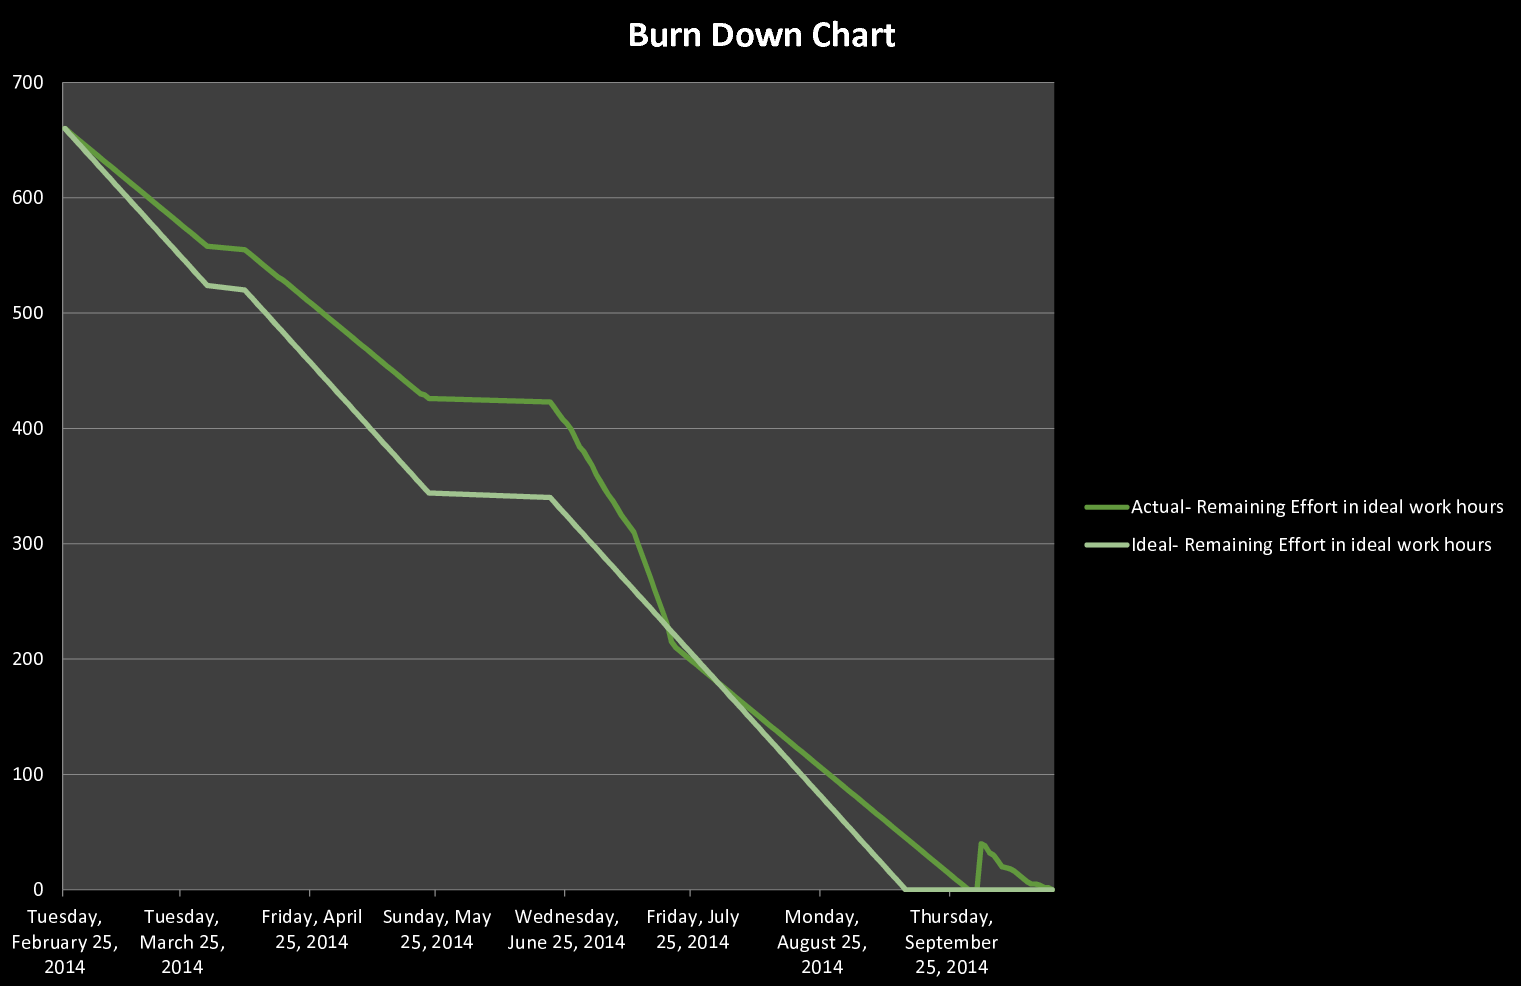
\includegraphics[scale=0.6]{../Images_Docs/Burn.png}}
\caption{Burn Down Chart}
\end{figure}


\begin{figure}[H]
\centering	
\framebox{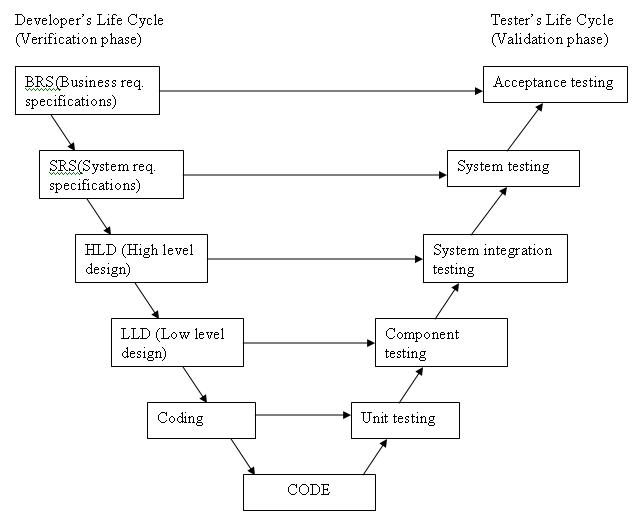
\includegraphics[scale=0.75]{../Images_Docs/model.jpg}}
\caption{V-Model Development Model}
\end{figure}

\end{document}